\documentclass{standalone}

\usepackage{tikz}
\usetikzlibrary{shapes, positioning, fit, backgrounds, arrows.meta}

\begin{document}
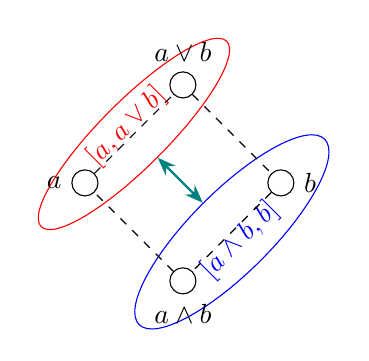
\begin{tikzpicture}[ele/.style = {circle, draw}, 
  ord/.style = {draw, dashed},
sublattice/.style = {draw, ellipse, inner sep = 5pt}]
  \node (aorb) [ele, label = {above: $a \lor b$}] {};
  \node (a) [ele, below left = of aorb, label = {left: $a$}] {};
  \node (b) [ele, below right = of aorb, label = {right: $b$}] {};
  \node (aandb) [ele, below right = of a, label = {below: $a \land b$}] {};

  \path (aandb) edge[ord] (a)
  	(a) 	edge[ord] (aorb)
	(aorb)  edge[ord] (b)
	(b)	edge[ord] (aandb);

  \begin{pgfonlayer}{background}
    \node (aab) [red, sublattice, rotate fit = 45, fit = (a) (aorb)] {$[a, a \lor b]$};
    \node (abb) [blue, sublattice, rotate fit = 45, fit = (b) (aandb)] {\\$[a \land b, b]$};
  \end{pgfonlayer}

  \draw [>=Stealth, <->, teal, thick] (aab) to (abb);
\end{tikzpicture}
\end{document}